This section presents our work with a content-based filter for
recommending movies related to another selected movie,
by defining some similarity metric supported by its features.

% get k=10 related movies
% -> get all movies
% -> for each movie, using certain criteria, generate a similarity coefficient (e.g. using cosine similarity)
% -> sort and get top k=10
\subsection*{Comparison}
Selected a movie, we define a similarity function for comparing it with every other movie in the dataset.
We consider two different approaches:
\begin{enumerate}
    \item The description of a movie already tells a lot about it; so, the first approach is taking the description string as the feature to compare (after applying TF-IDF on it).
    \item The second approach is making a "soup" of different features of a movie that we consider relevant for describing it.
\end{enumerate}
For both alternatives, the chosen objects of comparison from both the selected movie and the comparing one are sent as input vectors to a cosine similarity function,
which actually is the distance in polar coordinates for the dot product between both vectors:

\begin{center}
    \( cosine\_similarity = 
        \frac{movie_1 \cdotp movie_2}{\lVert movie_1 \rVert \lVert movie_2 \rVert}
    \)\\
\end{center}

\begin{center}
    \captionsetup{type=figure}
    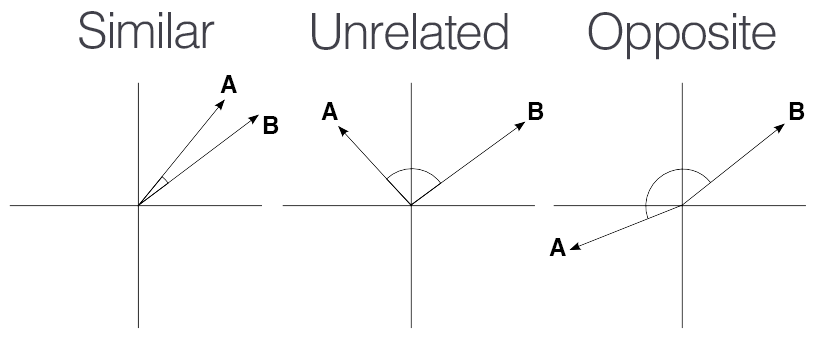
\includegraphics[width=250px]{images/cb-cos.png}
    \captionof{figure}{Graphic Representation of Cosine Similarity}
\end{center}

\subsection*{Implementation}
For a certain movie, we use the Cosine Similarity function between it and every other movie, generating a score for each pair.
Then, we sort them descending by said score, and finally take the top 10 movies. They are the 10 recommended movies, given the first one.
% TODO: show result of the function (image)
% TODO: caching?
